\chapter{Resultados}

\begin{figure}[H]
    \centering
    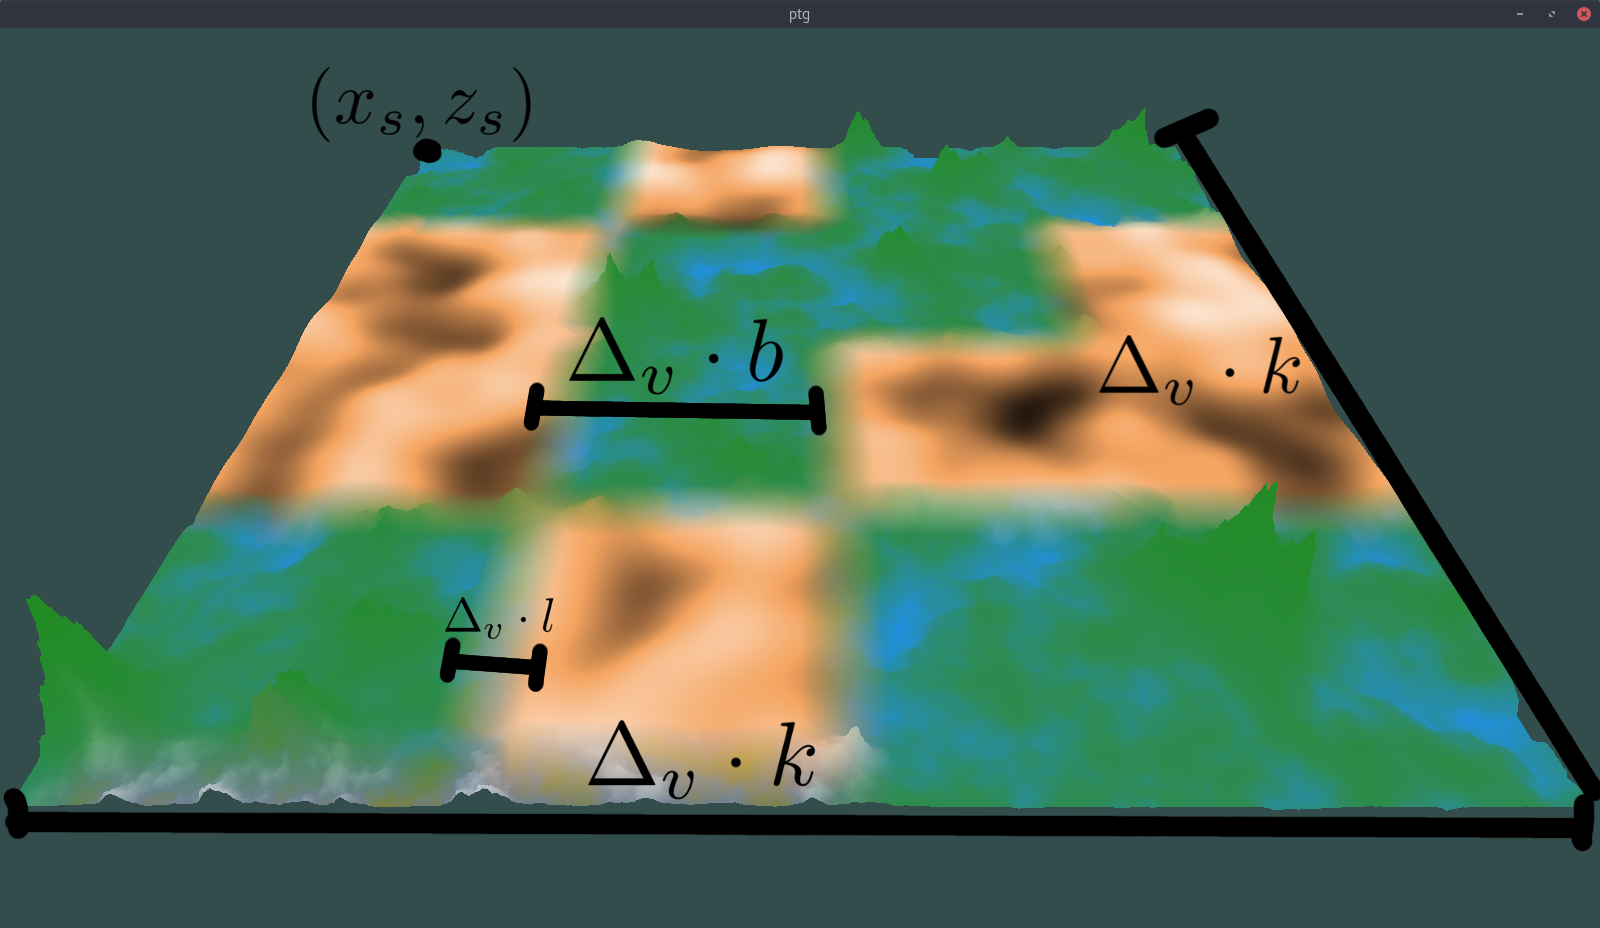
\includegraphics[width=0.75\textwidth]{figuras/resultados/sseditada.png}
    \caption{sseditada}
    \label{fig:sseditada}
\end{figure}


\begin{figure}[H]
    \centering
    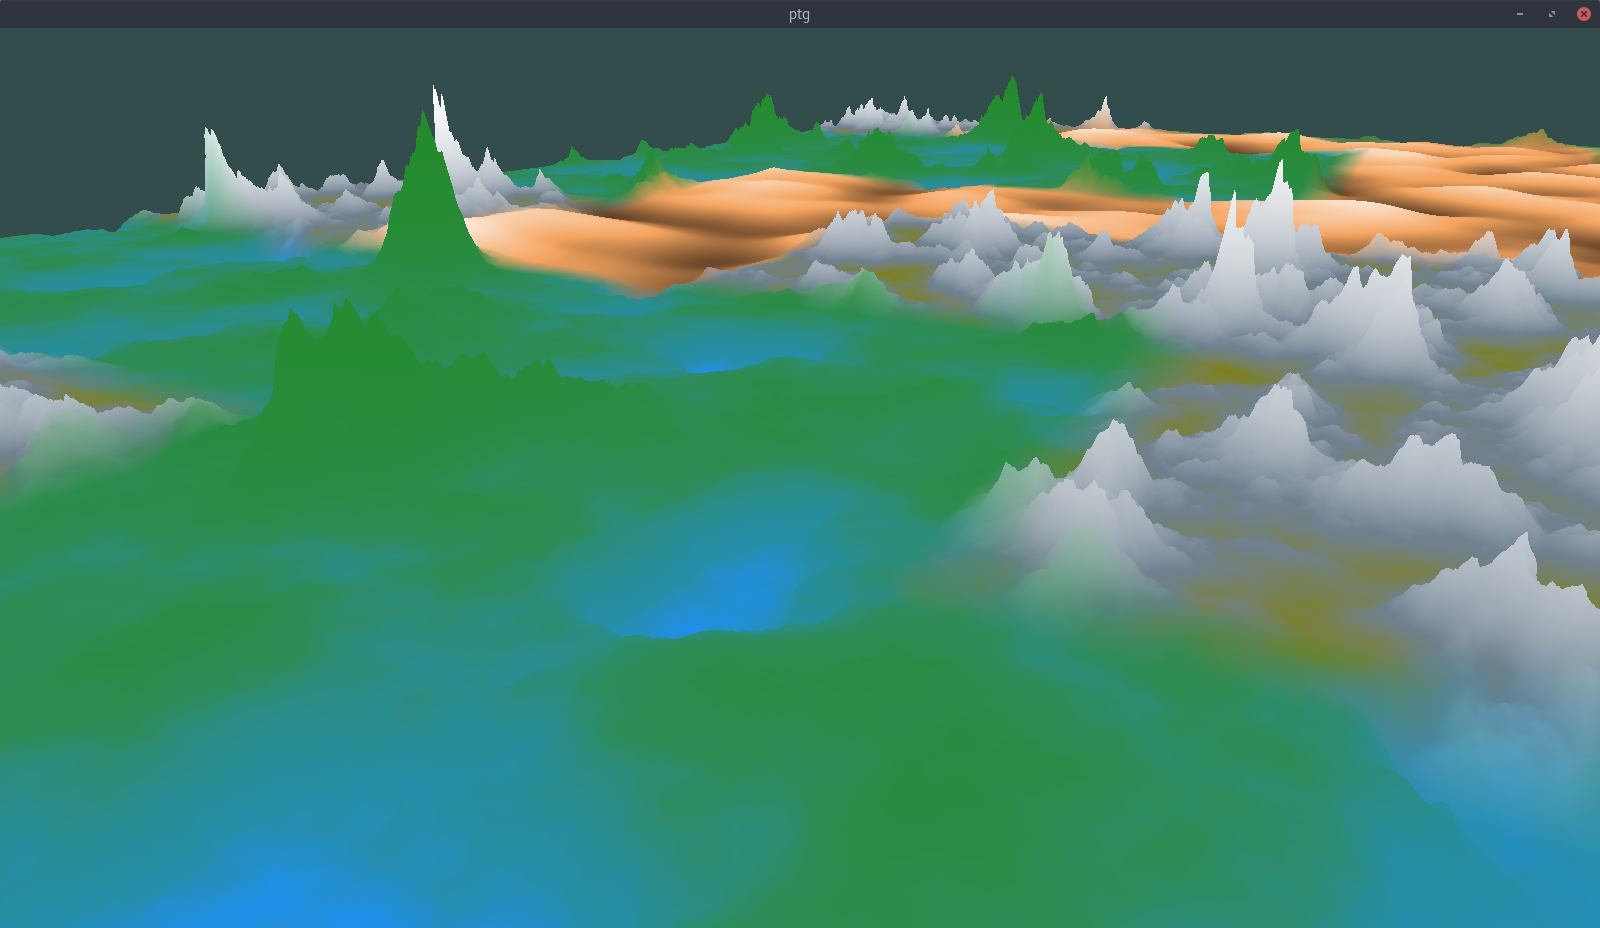
\includegraphics[width=0.5\textwidth]{figuras/ssFinalResult.png}
    \caption{Resultado final}
    \label{fig:ssFinalResult}
\end{figure}

\begin{figure}[H]
     \centering
     \subfloat[][$b = 260$]{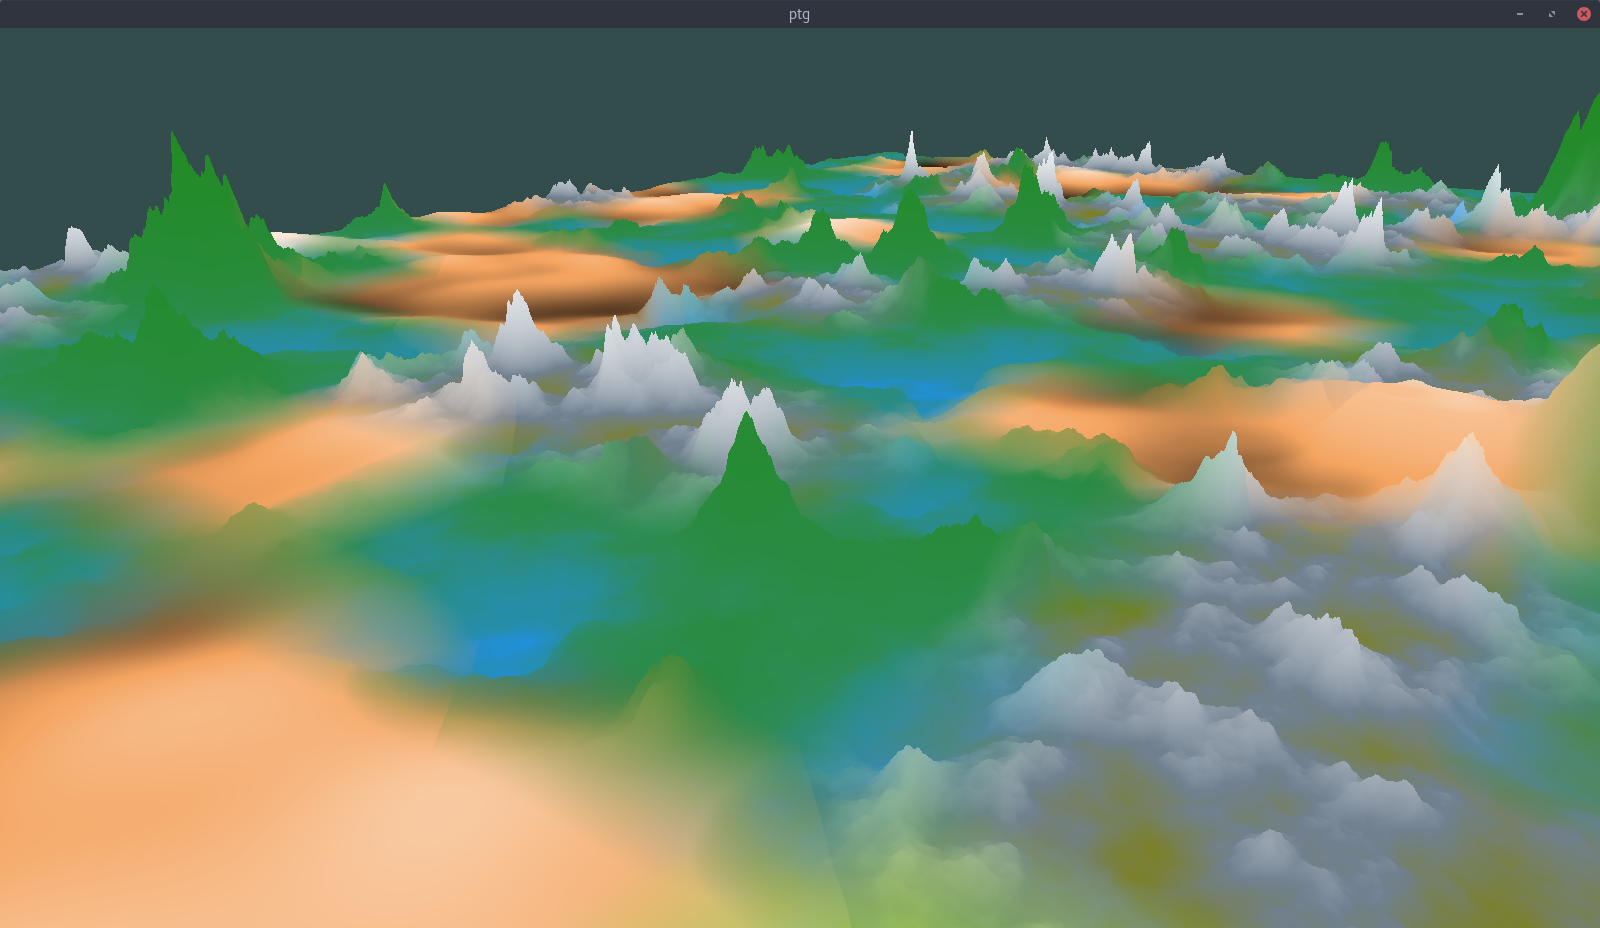
\includegraphics[width=0.48\textwidth]{figuras/resultados/b/resultSeed3Deltav05k2048b260l128.png}\label{fig:b260}}\hspace{0.1cm}
     \subfloat[][$b = 512$]{\includegraphics[width=0.48\textwidth]{figuras/resultados/b/resultSeed3Deltav05k2048b512l128.png}\label{fig:b512}}\\
     \subfloat[][$b = 1024$]{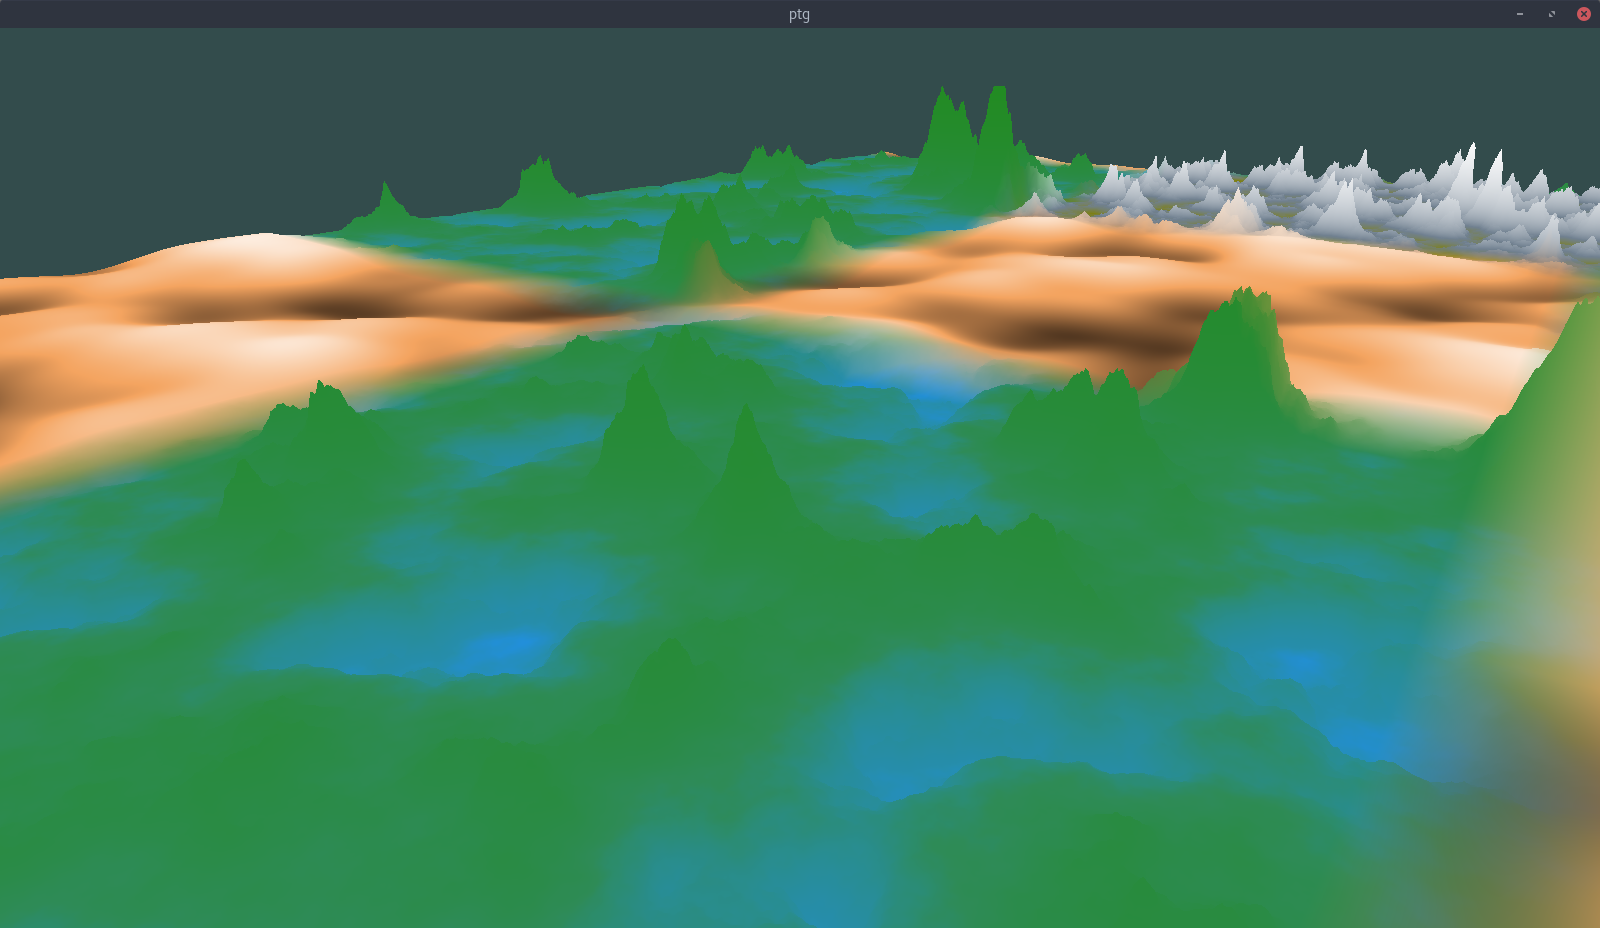
\includegraphics[width=0.48\textwidth]{figuras/resultados/b/resultSeed3Deltav05k2048b1024l128.png}\label{fig:b1024}}\hspace{0.1cm}
     \subfloat[][$b = 1500$]{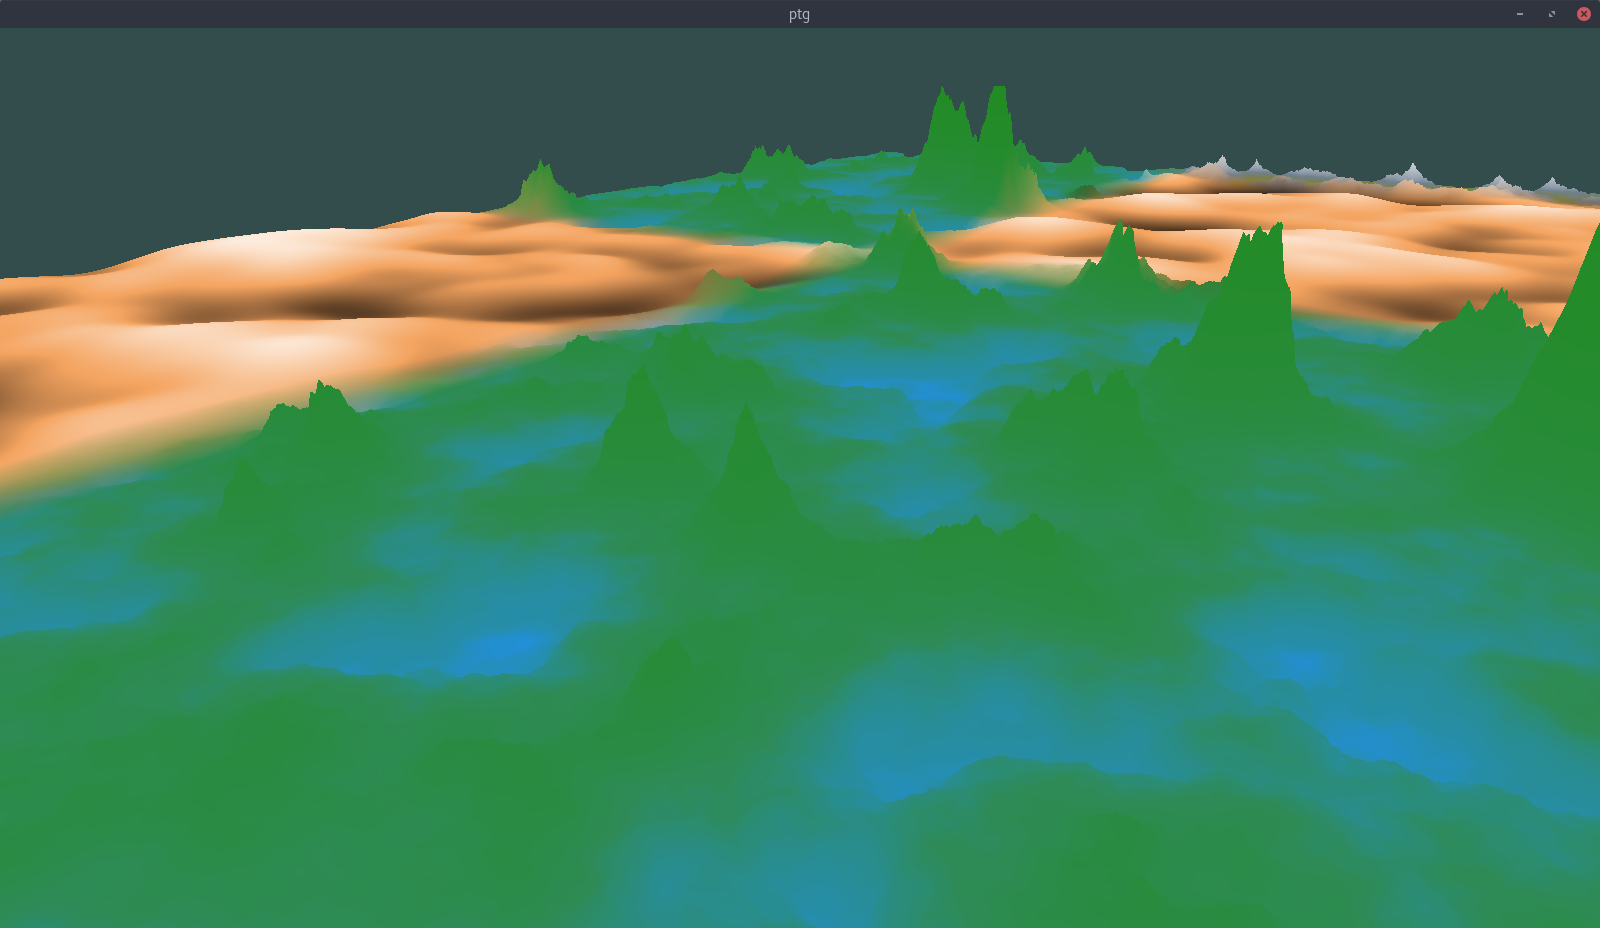
\includegraphics[width=0.48\textwidth]{figuras/resultados/b/resultSeed3Deltav05k2048b1500l128.png}\label{fig:b1500}}
     
     \caption{Tamanho de cada Bioma.}
     
     \label{fig:biomeComp}
     % usar \hspace{0.1cm}, é gambiarra mas funciona
\end{figure}

\begin{figure}[H]
     \centering
     \subfloat[][$l = 2$]{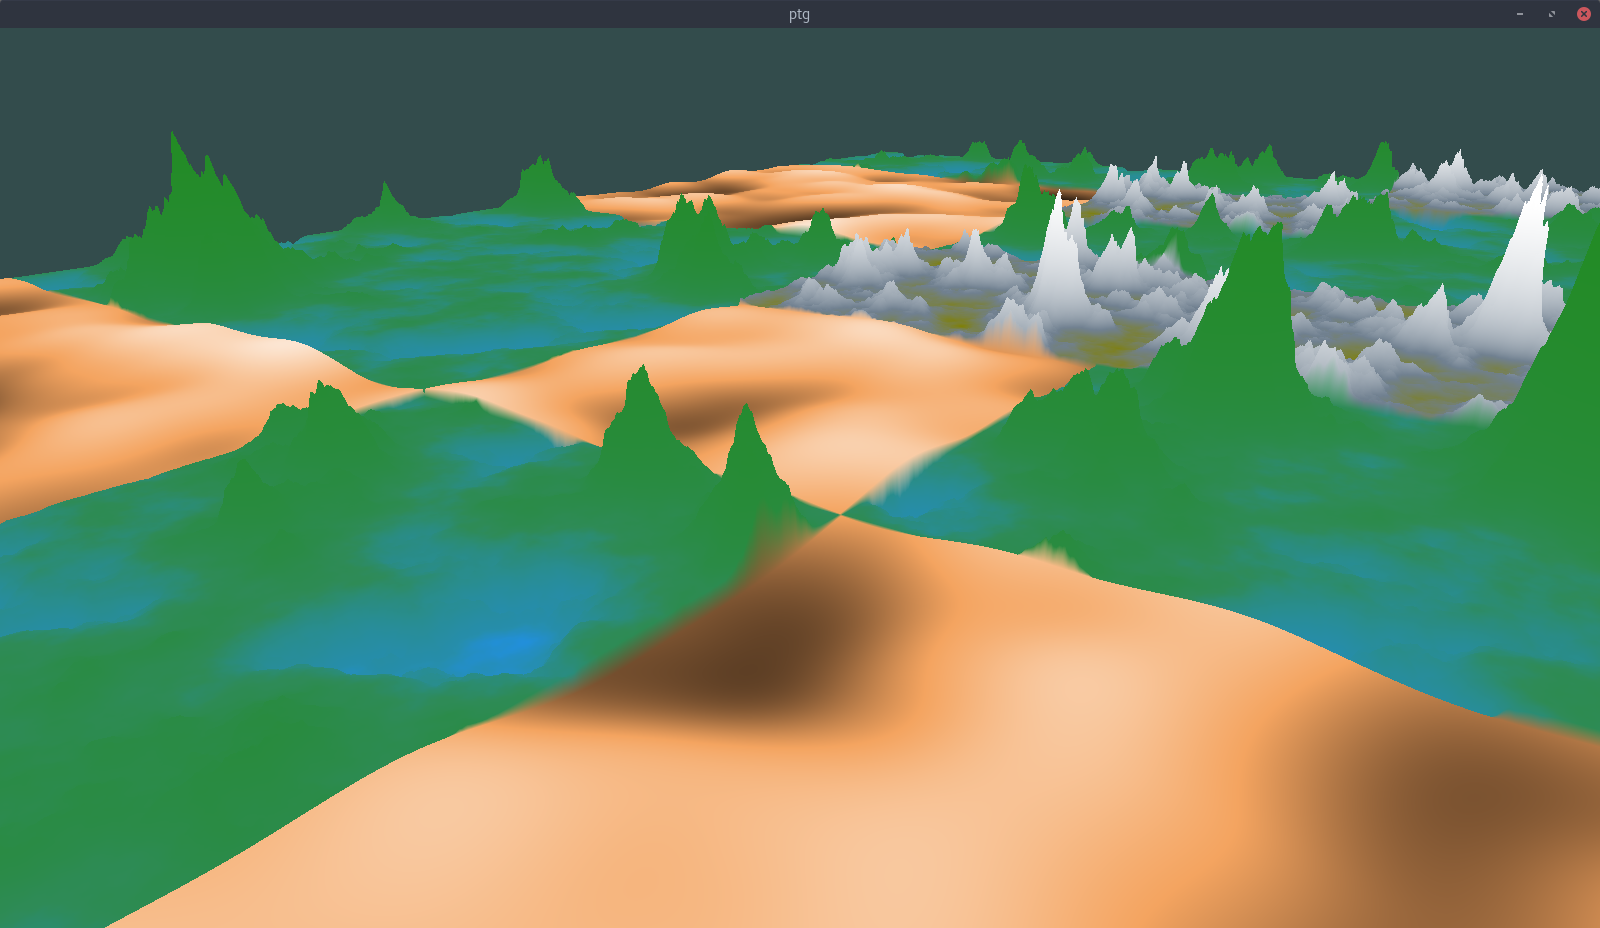
\includegraphics[width=0.48\textwidth]{figuras/resultados/l/resultSeed3Deltav05k2048b512l2.png}\label{fig:l2}}\hspace{0.1cm}
     \subfloat[][$l = 64$]{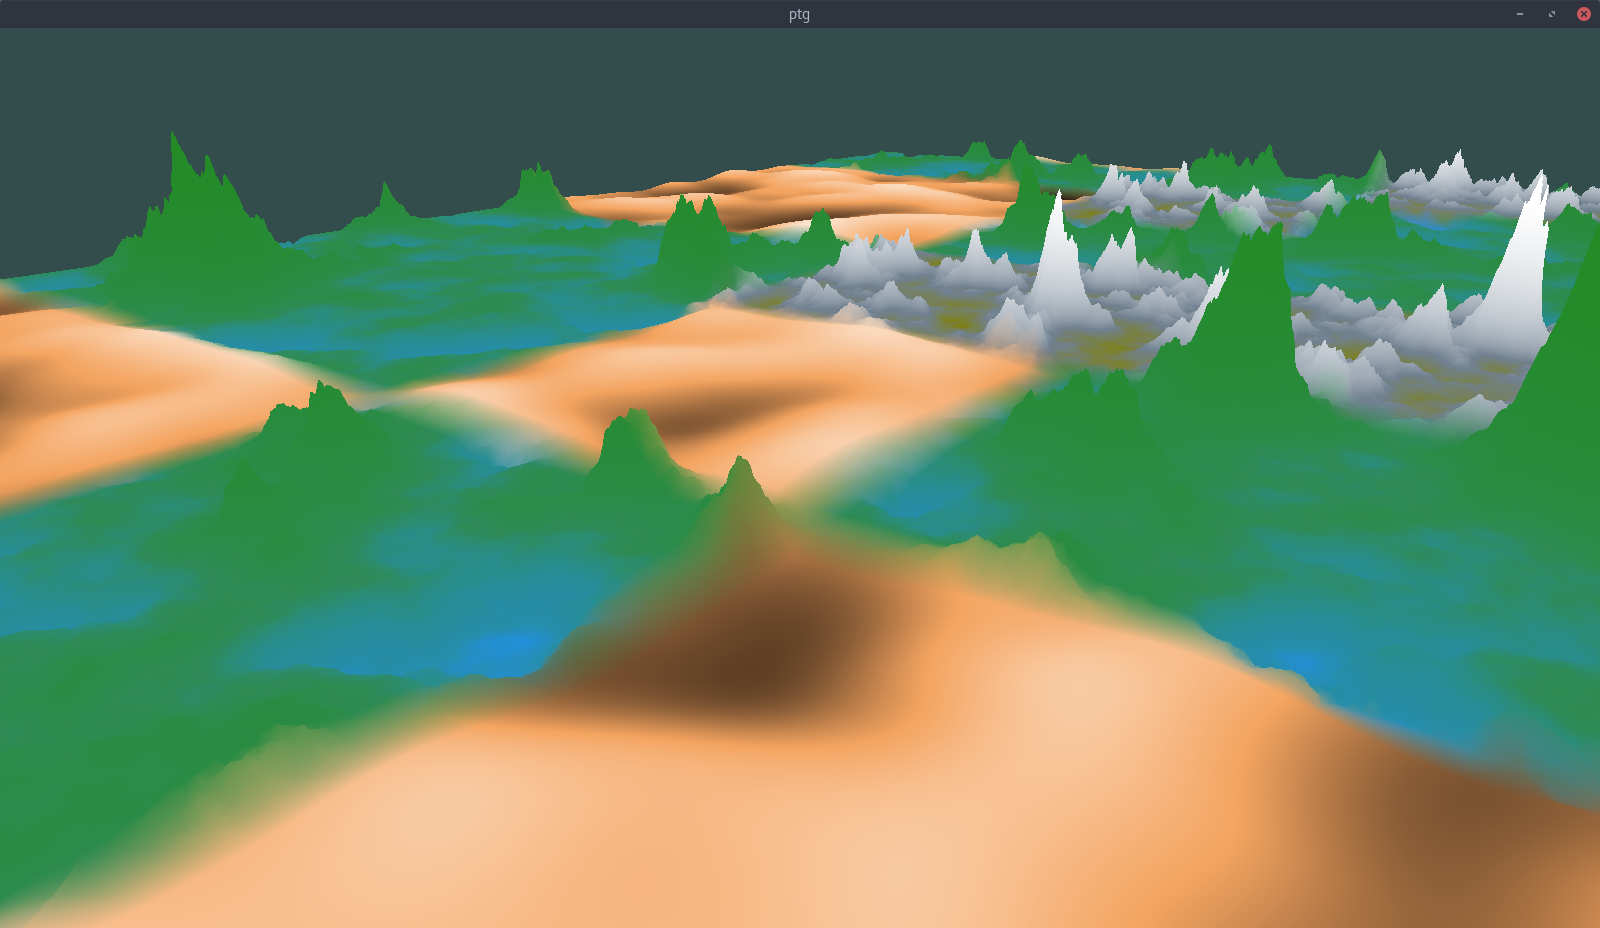
\includegraphics[width=0.48\textwidth]{figuras/resultados/l/resultSeed3Deltav05k2048b512l64.png}\label{fig:l64}}\\
     \subfloat[][$l = 128$]{\includegraphics[width=0.48\textwidth]{figuras/resultados/l/resultSeed3Deltav05k2048b512l128.png}\label{fig:l128}}\hspace{0.1cm}
     \subfloat[][$l = 256$]{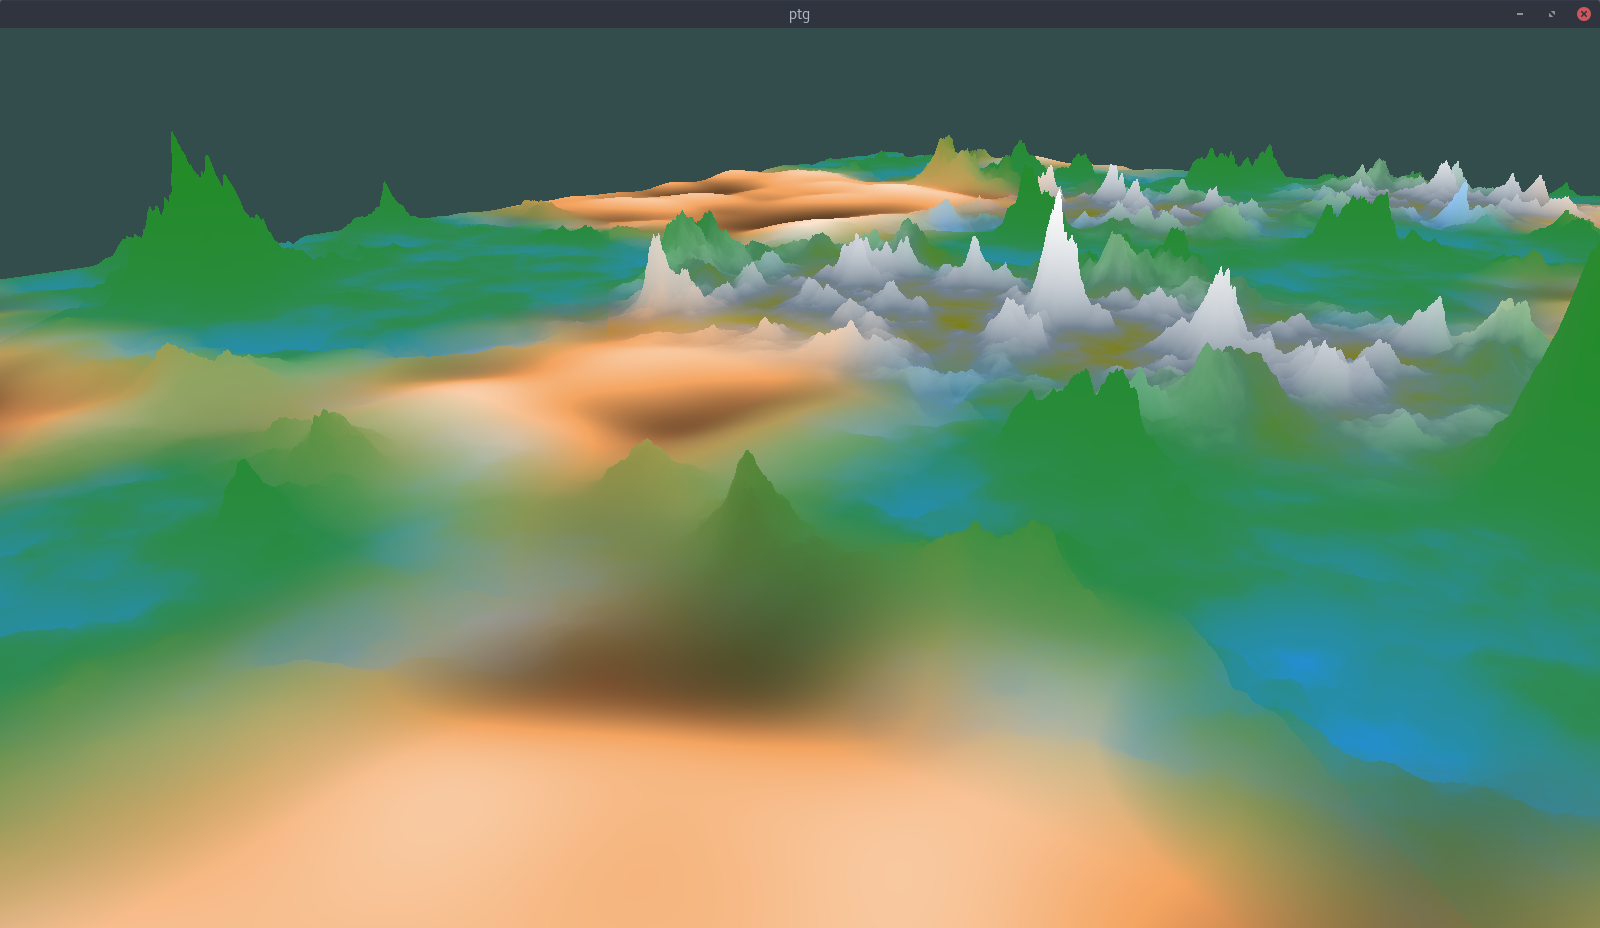
\includegraphics[width=0.48\textwidth]{figuras/resultados/l/resultSeed3Deltav05k2048b512l256.png}\label{fig:l256}}
     
     \caption{Alcance da fronteira.}
     
     \label{fig:lenghBioComp}
     % usar \hspace{0.1cm}, é gambiarra mas funciona
\end{figure}

\begin{figure}[H]
     \centering
     \subfloat[][$seed = 1$]{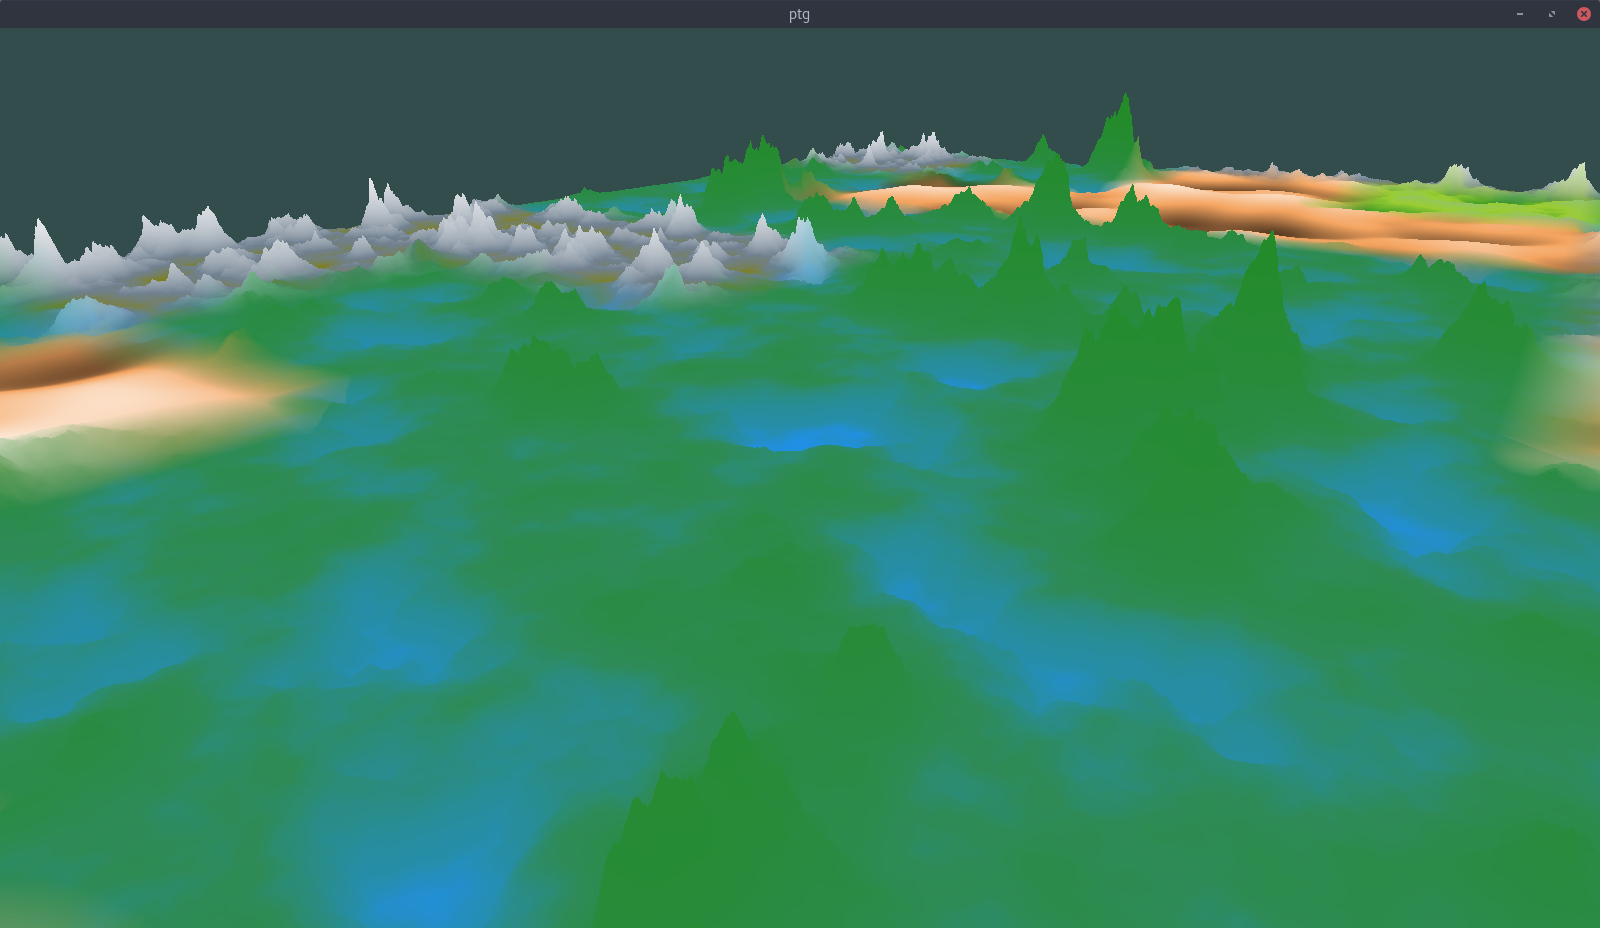
\includegraphics[width=0.48\textwidth]{figuras/resultados/seed/resultSeed1Deltav05k2048b512l128.png}\label{fig:seed1}}\hspace{0.1cm}
     \subfloat[][$seed = 2$]{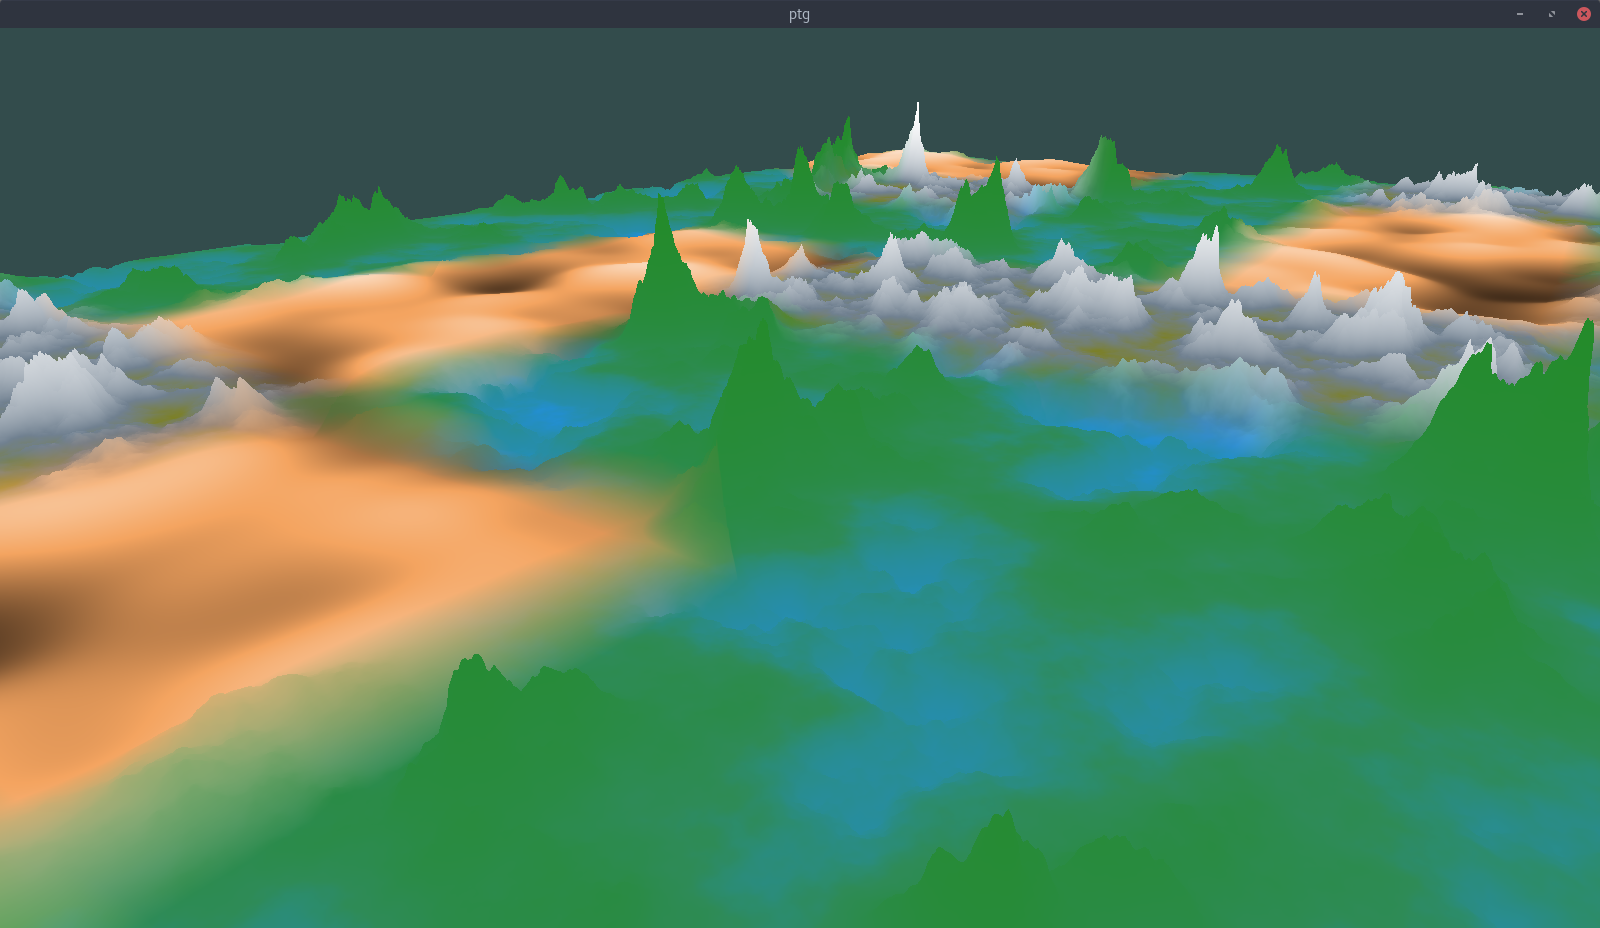
\includegraphics[width=0.48\textwidth]{figuras/resultados/seed/resultSeed2Deltav05k2048b512l128.png}\label{fig:seed2}}
     
     \caption{Semente para o motor de números pseudo aleatórios.}
     
     \label{fig:seedComp}
     % usar \hspace{0.1cm}, é gambiarra mas funciona
\end{figure}